\documentclass[letterpaper,12pt,fleqn]{article}
\usepackage{matharticle}
\usepackage{graphtheory}
\pagestyle{empty}
\begin{document}
\section*{1.1: Graphs and Graph Models}

\begin{enumerate}
\item What is a logical question to ask in Example 1.1?  Answer the question.

  Given ten editors on seven committees, determine how to schedule committee sessions into three time slots such
  that any two committees that meet during the same time slot do not have any common members.  The graph for this
  problem represents the committees with nodes.  If any two committees have a common member, then their
  corresponding nodes are adjacent.  Thus, the solution to the problem is to partition the nodes into three
  independent sets.  This is an example of a node coloring problem.  To solve this problem, use a greedy coloring
  algorithm:

  \begin{minipage}{3in}
    \begin{tikzpicture}
      \colorlet{g1}{green!25!white}
      \colorlet{g2}{blue!25!white}
      \colorlet{g3}{red!25!white}
      \cycleNnodes{7}{(0,0)}{2cm}{90}{}
      \begin{scope}[every node/.style=labeled node]
        \foreach \i/\c in {1/g1, 2/g2, 3/g3, 4/g1, 5/g2, 6/g2, 7/g3} {
          \node [fill=\c] (c\i) at (\i) {\(c_{\i}\)};
        }
      \end{scope}
      \draw (c1) edge (c2) edge (c3) edge (c5) edge (c7);
      \draw (c2) edge (c3) edge (c4) edge (c7);
      \draw (c3) edge (c4) edge (c5);
      \draw (c4) edge (c5) edge (c6) edge (c7);
      \draw (c6) edge (c7);
    \end{tikzpicture}
  \end{minipage}
  \begin{minipage}{3in}
    \begin{tabular}{c|c}
      slot & committees \\
      \hline
      1 & \(c_1, c_4\) \\
      2 & \(c_2, c_5, c_6\) \\
      3 & \(c_3, c_7\)
    \end{tabular}
  \end{minipage}

  \bigskip

\item Create an example of your own similar to Example 1.1 with nine editors and eight committees and then draw the
  corresponding graph.

  \bigskip

  \begin{minipage}{2in}
    \begin{tabular}{c|c}
      committee & members \\
      \hline
      1 & \(1,2,7,8\) \\
      2 & \(3,4\) \\
      3 & \(1,7\) \\
      4 & \(3,4,5\) \\
      5 & \(5,6\) \\
      6 & \(2,7,8\) \\
      7 & \(4,9\) \\
      8 & \(5,6\)
    \end{tabular}
  \end{minipage}
  \begin{minipage}{2.25in}
    \begin{tikzpicture}
      \colorlet{g1}{green!25!white}
      \colorlet{g2}{blue!25!white}
      \colorlet{g3}{red!25!white}
      \cycleNnodes{8}{(0,0)}{2cm}{90}{}
      \begin{scope}[every node/.style={labeled node}]
        \foreach \i/\c in {1/g1, 2/g1, 3/g2, 4/g2, 5/g1, 6/g3, 7/g3, 8/g3} {
          \node [fill=\c] (c\i) at (\i) {\(c_{\i}\)};
        }
      \end{scope}
      \draw (c1) edge (c3) edge (c6);
      \draw (c2) edge (c4) edge (c7);
      \draw (c3) edge (c6);
      \draw (c4) edge (c5) edge (c7) edge (c8);
      \draw (c5) edge (c8);
    \end{tikzpicture}
  \end{minipage}
  \begin{minipage}{1.75in}
    \begin{tabular}{c|c}
      slot & committees \\
      \hline
      1 & \(c_1, c_2, c_5\) \\
      2 & \(c_3, c_4\) \\
      3 & \(c_6, c_7, c_8\)
    \end{tabular}
  \end{minipage}

  \bigskip

\item Let \(S=\set{2,3,4,7,11,13}\).  Draw the graph \(G\) whose vertex set is \(S\) and such that \(ij\in E(G)\) for
  \(i,j\in S\) if \(i+j\in S\) or \(\abs{i-j}\in S\).

  \bigskip
  
  \begin{center}
    \begin{tikzpicture}
      \begin{scope}[every node/.style={labeled node}]
        \cycleVnodes{\(2\),\(3\),\(4\),\(7\),\(11\),\(13\)}{(0,0)}{2cm}{90}{n}
      \end{scope}
      \draw (n1) edge (n3) edge (n5) edge (n6);
      \draw (n2) edge (n3) edge (n4);
      \draw (n3) edge (n4) edge (n5);
      \draw (n4) edge (n5);
      \draw (n5) edge (n6);
    \end{tikzpicture}
  \end{center}

  \bigskip

\item Let \(S=\set{-6,-3,0,3,6}\).  Draw the graph \(G\) whose vertex set is \(S\) and such that \(ij\in E(G)\) for
  \(i,j\in S\) if \(i+j\in S\) or \(\abs{i-j}\in S\).

  \bigskip
  
  \begin{center}
    \begin{tikzpicture}
      \begin{scope}[every node/.style={labeled node}]
        \completeV{\(-6\),\(-3\),\(0\),\(3\),\(6\)}{(0,0)}{2cm}{90}{}
      \end{scope}
    \end{tikzpicture}
  \end{center}

  \bigskip

\item Create your own set \(S\) of integers and draw the graph \(G\) whose vertex set is \(S\) and such that
  \(ij\in E(G)\) if \(i\) and \(j\) are related by some rule imposed on \(i\) and \(j\).

  \bigskip

  Let \(S=\set{1,2,5,6,7,9}\) and let \(ij\in E(G)\) if \(i+j\) is an even number.

  \bigskip
  
  \begin{center}
    \begin{tikzpicture}
      \begin{scope}[every node/.style={labeled node}]
        \cycleVnodes{\(1\),\(2\),\(5\),\(6\),\(7\),\(9\)}{(0,0)}{2cm}{90}{n}
      \end{scope}
      \draw (n1) edge (n3) edge (n5) edge (n6);
      \draw (n2) edge (n4);
      \draw (n3) edge (n5) edge (n6);
      \draw (n5) edge (n6);
    \end{tikzpicture}
  \end{center}

  \bigskip

\item Consider the twelve configurations \(c_1,c_2,\ldots,c_{12}\) in Figure 1.4.  For every two configurations
  \(c_i\) and \(c_j\), where \(1\le i,j\le12, i\ne j\), it may be possible to obtain \(c_j\) from \(c_i\) by first
  shifting one of the coins in \(c_i\) horizontally or vertically \emph{and} then interchanging the two coins.
  Model this by a graph \(F\) such that \(V(F)=\set{c_1,c_2,\ldots,c_{12}}\) and \(c_ic_j\) is an edge of \(F\) if
  \(c_i\) and \(c_j\) can be transformed into each other by this two step process.

  \bigskip
  
  \begin{center}
    \begin{tikzpicture}
      \begin{scope}[every node/.style={labeled node}]
        \cycleVnodes{\(c_1\),\(c_2\),\(c_3\),\(c_4\),\(c_5\),\(c_6\),
          \(c_7\),\(c_8\),\(c_9\),\(c_{10}\),\(c_{11}\),\(c_{12}\)}{(0,0)}{2in}{90}{c}
      \end{scope}
      \draw (c1) edge (c5) edge (c6) edge (c8) edge (c9);
      \draw (c2) edge (c7) edge (c10);
      \draw (c3) edge (c7) edge (c10);
      \draw (c4) edge (c8) edge (c9) edge (c11) edge (c12);
      \draw (c5) edge (c10);
      \draw (c6) edge (c10);
      \draw (c7) edge (c11) edge (c12);
    \end{tikzpicture}
  \end{center}

  \bigskip

\item Following Example 1.4,
  \begin{enumerate}
  \item give an example of ten 3-letter words, none of which are mentioned in Example 1.4 and whose corresponding
    word graph has at least six edges.  Draw this graph.

    \bigskip

    \begin{center}
      \begin{tikzpicture}
        \node (tab) {TAB};
        \node (bat) [right=of tab] {BAT};
        \node (bet) [right=3cm of bat] {BET};
        \node (get) [right=of bet] {GET};
        \node (bit) [above=of bat] {BIT};
        \node (but) [above=of bet] {BUT};
        \node (jet) [below=of bet] {JET};
        \node (far) [below=of bat] {FAR};
        \node (bar) [left=of far] {BAR};
        \node (fat) [right=of far] {FAT};
        \draw (tab) edge (bat);
        \draw (bar) edge (bat) edge (far);
        \draw (bit) edge (bat) edge (but) edge (bet);
        \draw (bat) edge (fat) edge (but) edge (bet);
        \draw (far) edge (fat);
        \draw (but) edge (bet);
        \draw (bet) edge (jet) edge (get);
        \draw (jet) edge (get);
      \end{tikzpicture}
    \end{center}

    \bigskip

  \item give a set of five 3-letter words whose word graph is shown in Figure 1.11 (with the vertices appropriately
    labeled).

    \bigskip

    \begin{center}
      \begin{tikzpicture}[node distance=2cm]
        \pathV{TAB,BAT,BET,GET,GEM}{(0,0)}{right}{w}
      \end{tikzpicture}
    \end{center}

    \bigskip

  \item give a set of five 3-letter words whose word graph is shown in Figure 1.12 (with the vertices appropriately
    labeled).

    \bigskip

    \begin{center}
      \begin{tikzpicture}
        \cycleV{TAB,BAT,CAT,CAN,TAN}{(0,0)}{2cm}{90}{w}
      \end{tikzpicture}
    \end{center}
  \end{enumerate}

  \bigskip

\item Let \(S\) be a finite set of 3-letter and/or 4-letter words.  In this case, the word graph \(G(S)\) of \(S\)
  is that graph whose vertex set is \(S\) and such that two vertices (words) \(w_1\) and \(w_2\) are adjacent if
  either (1) or (2) below occurs:
  \begin{enumerate}[label=(\arabic*)]
  \item one of the words can be obtained from the other by replacing one letter by another letter.
  \item \(w_1\) is a 3-letter word and \(w_2\) is a 4-letter word and \(w_2\) can be obtained from \(w_1\) by the
    insertion of a single letter (anywhere, including the beginning or the end) into \(w_1\).
  \end{enumerate}
  \begin{enumerate}
  \item Find six sets \(S_1,S_2,\ldots,S_6\) of 3-letter and/or 4-letter words so that for each integer \(i\)
    \((1\le i\le6)\) the graph \(G_i\) of Figure 1.13 is the word graph of \(S_i\).
    \begin{center}
      \begin{tikzpicture}[node distance=2cm]
        \pathV{ART,CART,CARD,HARD,ART}{(0,0)}{right}{}
        \node [below=0.25in of 3] {\(G_1\)};
      \end{tikzpicture}

      \bigskip
      
      \begin{tikzpicture}
        \starV{BID,BIRD,BAD,BIT}{(0,0)}{1in}{150}{}
        \node [below=0.25in of 4] {\(G_2\)};
      \end{tikzpicture}

      \bigskip
      
      \begin{tikzpicture}
        \starV{BID,BUD,BAD,BIRD}{(0,0)}{1in}{150}{}
        \draw (2) edge (3);
        \node [below=0.25in of 4] {\(G_3\)};
      \end{tikzpicture}

      \bigskip
      
      \begin{tikzpicture}
        \cycleV{BAD,BUD,BUT,BAT}{(0,0)}{1in}{135}{}
        \draw (2) edge (3);
        \node [below=0.25in] at ($ (3)!0.5!(4) $) {\(G_4\)};
      \end{tikzpicture}

      \bigskip
      
      \begin{tikzpicture}
        \cycleV{MAID,AID,MID,MAD}{(0,0)}{1in}{135}{}
        \draw (1) edge (3);
        \node [below=0.25in] at ($ (3)!0.5!(4) $) {\(G_5\)};
      \end{tikzpicture}
      \bigskip
      
      \begin{tikzpicture}
        \completeV{BIT,BUT,BET,BAT}{(0,0)}{1in}{135}{}
        \node [below=0.25in] at ($ (3)!0.5!(4) $) {\(G_6\)};
      \end{tikzpicture}
    \end{center}

    \bigskip

  \item For another graph \(H\) (of your choice), determine whether \(H\) is a word graph of some sort.

    \bigskip

    \begin{tikzpicture}[node distance=2cm]
      \bipartiteVnodes{BAR,BOAR,OAR}{(0,0)}{right}{v}{GOAT,BOAT,BOLT}{(0,-2cm)}{right}{w}
      \draw (v1) -- (v2) -- (v3);
      \draw (w1) -- (w2) -- (w3);
      \draw (v2) -- (w2);
    \end{tikzpicture}
  \end{enumerate}

  \bigskip

\item Define a word graph differently from the word graphs defined in Example 1.4 and Exercise 1.8 and illustrate
  your definition.

  Let \(S\) be a finite set of 3-letter words.  The word graph \(G(S)\) of \(S\) is that graph whose vertex set
  is \(S\) and such that two vertices (words) \(w_1\) and \(w_2\) are adjacent if either (1) or (2) below occurs:
  \begin{enumerate}[label=(\arabic*)]
  \item one can be obtained from the other by replacing one letter by another letter.
  \item one is an anagram of the other.
  \end{enumerate}

  \bigskip

  \begin{center}
    \begin{tikzpicture}[node distance=2cm]
      \cycleV{ART,TAR,CAR,ARC}{(0,0)}{1in}{135}{}
    \end{tikzpicture}
  \end{center}

  \bigskip

\item Figure 1.14 illustrates the traffic lanes at the intersection of two streets.  When a vehicle approaches this
  intersection, it could be in one of the seven lanes: \(L_1,L_2,\ldots,L_7\).  Draw a graph \(G\) that models this
  situation, where \(V(G)=\set{L_1,L_2,\ldots,L_7}\) and where two vertices are joined by an edge if vehicles in
  these two lanes cannot safely enter this intersection at the same time.

  \bigskip

  \begin{center}
    \begin{tikzpicture}[every node/.style=labeled node]
      \cycleVnodes{\(L_1\),\(L_2\),\(L_3\),\(L_4\),\(L_5\),\(L_6\),\(L_7\)}{(0,0)}{1in}{90}{L};
      \draw (L1) edge (L3) edge (L4) edge (L5) edge (L6);
      \draw (L2) edge (L3) edge (L4);
      \draw (L3) edge (L5) edge (L7);
      \draw (L4) edge (L5) edge (L6);
      \draw (L5) edge (L6) edge (L7);
    \end{tikzpicture}
  \end{center}
\end{enumerate}

\end{document}
